\section{Battleship Circuits}

\begin{frame}{Circom: A Language for Zero-Knowledge Circuits}
    \begin{itemize}
        \item \defn{\Glsxtrfull{dsl}} written specifically for \glsxtrfullpl{zkp}.
        \item Requires game rules to be expressed using \defn{arithmetic constraints}.
        \item Uses \defn{Signals} (wires carrying values) and \defn{Components}.
        \item Compiles into a \glsxtrfull{r1cs}.
    \end{itemize}
\end{frame}

\begin{frame}{Circom $\rightarrow \groth$ Pipeline}
    \begin{figure}
        \centering
        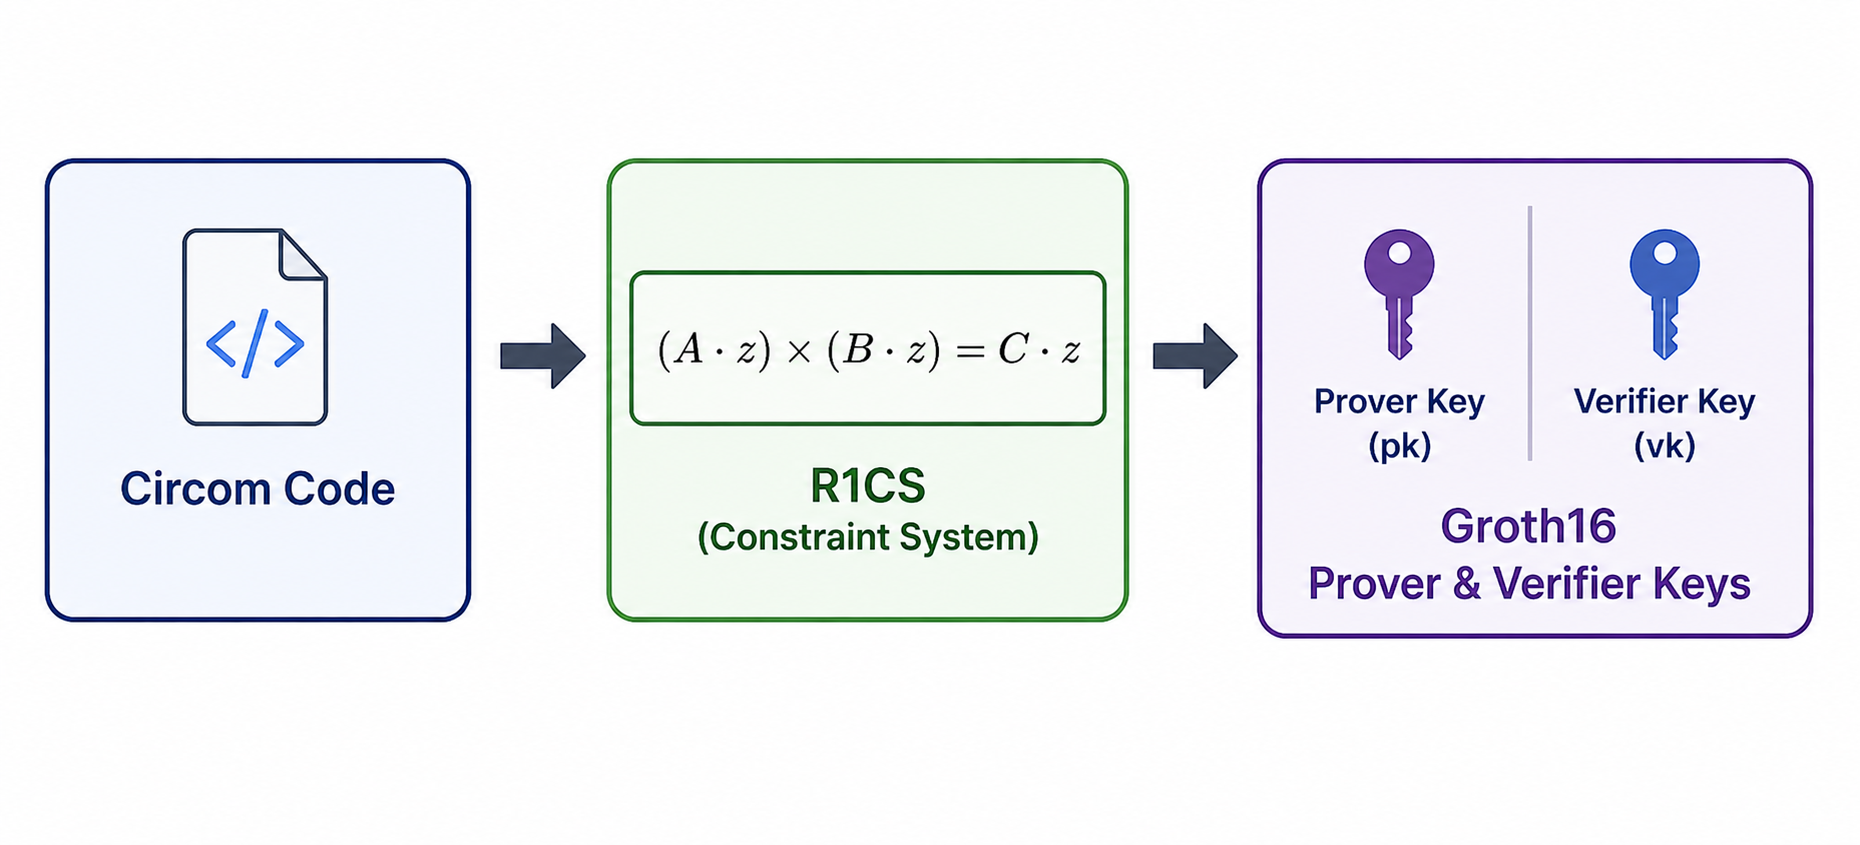
\includegraphics[width=0.7\textwidth]{Images/circom_pipeline.png}
    \end{figure}
    \begin{enumerate}
        \item \defn{Circom (The Compiler)}
        \begin{itemize}
            \item Outputs a \glsxtrshort{r1cs}.
            \item Generates a \defn{witness generator}.
        \end{itemize}
        \item \defn{snarkjs (The Prover \& Verifier)}
        \begin{itemize}
            \item Takes the \glsxtrshort{r1cs} and creates \defn{proving} and \defn{verification keys}.
            \item Applies the \defn{Groth16} protocol to the witness.
        \end{itemize}
    \end{enumerate}
\end{frame}

\begin{frame}[fragile]{Circuit 1: Board Verification}
    \begin{columns}<1->
        \column{0.5\textwidth}
        \begin{itemize}
            \item \defn{Private inputs:} Ship $\del{x, y}$ coordinates and a private salt.
            \item \defn{Public output:} A $\poseidon$ hash (commitment).
            \item Circuit enforces bounds, overlaps, and valid shapes.
        \end{itemize}
        \column{0.5\textwidth}
        \begin{minted}[fontsize=\tiny]{javascript}
component eqX[N][N];
component eqY[N][N];

for (var i = 0; i < N; i++) {
    for (var j = i + 1; j < N; i++) {
        eqX[i][j] = IsEqual();
        eqX[i][j].in[0] <== privShipX[i];
        eqX[i][j].in[1] <== privShipX[j];
        
        eqY[i][j] = IsEqual();
        eqY[i][j].in[0] <== privShipY[i];
        eqY[i][j].in[1] <== privShipY[j];
        
        eqX[i][j].out * eqY[i][j].out === 0;
    }
}
        \end{minted}
        \vspace{-1em}
        \begin{uncoverenv}<+->
            \begin{minted}[fontsize=\tiny]{javascript}
component hasher = Poseidon(15);

for (var i = 0; i < N; i++) {
    hasher.inputs[i] <== privShipX[i];
    hasher.inputs[i + N] <== privShipY[i];
}

hasher.inputs[2 * N] <== privSalt;
pubCommitment <== hasher.out;
            \end{minted}
        \end{uncoverenv}
    \end{columns}
\end{frame}

\begin{frame}[fragile]{Circuit 2: Proving the Attack}
    \begin{columns}<1->
        \column{0.5\textwidth}
        \begin{itemize}
            \item \defn{Private inputs:} Ship $\del{x, y}$ coordinates and a private salt (same).
            \item \defn{Public inputs:} Player's guess, opponent board commitment, reported result $z \in \set{\hit, \miss}$.
            \item The circuit enforces the unchanged opponent board state and that the reported result is accurate.
        \end{itemize}
        \column{0.5\textwidth}
        \begin{minted}[fontsize=\tiny]{javascript}
component hasher = Poseidon(2 * N + 1);

for (var i = 0; i < N; i++) {
    hasher.inputs[i] <== privShipX[i];
    hasher.inputs[i + N] <== privShipY[i];
}

hasher.inputs[2 * N] <== privSalt;
pubCommitment === hasher.out;
        \end{minted}
        \vspace{-1em}
        \begin{uncoverenv}<+->
            \begin{minted}[fontsize=\tiny]{javascript}
signal hitAccumulator[N + 1];
hitAccumulator[0] <== 0;

for (var i = 0; i < N; i++) {
    eqX[i] = IsEqual();
    eqX[i].in[0] <== pubGuessX;
    eqX[i].in[1] <== privShipX[i];
    
    eqY[i] = IsEqual();
    eqY[i].in[0] <== pubGuessY;
    eqY[i].in[1] <== privShipY[i];

    hitMatch[i] <== eqX[i].out * eqY[i].out
    hitAccumulator[i + 1] <== hitAccumulator[i] + hitMatch[i];
}

pubReportedHit === hitAccumulator[N];
            \end{minted}
        \end{uncoverenv}
    \end{columns}
\end{frame}

\begin{frame}{Limitation}
    \begin{itemize}
        \item \defn{Poseidon capacity:} The Circom implementation is optimized for a maximum of 16 inputs.
        \item \defn{Coordinate cap:} Each ship square needs a coordinate $\del{x, y}$. Including the salt, we are therefore capped at 7 squares:
        \begin{equation*}
            \underbrace{2 \cdot 7}_{\del{x, y} \text{ coordinates}} + \underbrace{1}_{\text{salt}} \leq 16
        \end{equation*}
        
        \item \defn{Conflict:} Standard Battleship requires 5 ships totaling 17 squares.
        \item \defn{The fix?}
    \end{itemize}
\end{frame}
